\makeproblem{LNDASH}{Trò chơi LineDash}{1.0s}{1024 MB}

\begin{center}
    \begin{minipage}{\textwidth}
        \hrule
        \vspace{0.25cm}
        \noindent \textbf{Lưu ý đặc biệt:}
        
        Do có một số sự bất tương đồng giữa các nguồn thông tin, bài toán này hiện tồn tại hai phiên bản. Tại phiên bản hiện tại, giới hạn được thiết lập như sau:
        \begin{itemize}
            \item $0 \le L_i \le R_i \le N$.
        \end{itemize}
        
        \noindent Thí sinh được khuyến khích thực hiện lời giải theo phiên bản \textbf{còn lại}. Đồng thời, nhằm đảm bảo tính công bằng trong việc chấm điểm, bài toán này sử dụng checker. Kết quả của thí sinh được tính là chính xác nếu sai số tuyệt đối hoặc tương đối so với đáp án không vượt quá $10^{-6}$.
        \vspace{0.25cm}
        \hrule
    \end{minipage}
\end{center}

Cho một nhân vật trong game di chuyển trên mặt phẳng tọa độ $Oxy$. Tại mỗi thời điểm, nhân vật thực hiện một trong ba loại hiệu lệnh sau:
\begin{itemize}
    \item \fbox{\texttt{/}} : di chuyển đến ô $(x+1, y+1)$
    \item \fbox{\texttt{-}} : di chuyển đến ô $(x+1, y)$
    \item \fbox{\texttt{\textbackslash}} : di chuyển đến ô $(x+1, y-1)$
\end{itemize}

Ban đầu (tại thời điểm $0$), hiệu lệnh là \fbox{\texttt{-}}. Có $N$ lần thay đổi tín hiệu, mỗi lần thay đổi tại thời điểm $C_i$, hiệu lệnh sẽ được chuyển thành một trong ba loại trên. Hiệu lệnh sau khi thay đổi sẽ được giữ nguyên cho đến lần thay đổi tiếp theo.

\medskip
\textbf{Yêu cầu:} Có $Q$ truy vấn, mỗi truy vấn thứ $i$ yêu cầu tính tổng quãng đường mà nhân vật đã di chuyển từ thời điểm $L_i$ đến $R_i$.

\bigskip
\textbf{Lưu ý:}
\begin{itemize}
    \item Tại thời điểm $t$, nhân vật thực hiện \textbf{1 bước di chuyển} theo hiệu lệnh tại thời điểm đó.  
    \item Khi tính tổng quãng đường từ $L_i$ đến $R_i$, chỉ tính các bước từ $L_i \to L_i+1, L_i+1 \to L_i+2, \dots, R_i-1 \to R_i$.  
    \item Thời điểm $R_i$ không sinh thêm bước đi.
\end{itemize}

Kết quả cần được làm tròn đến đúng \textbf{6 chữ số thập phân}.


\makesection{Input}
\begin{itemize}
    \item Dòng đầu tiên chứa ba số nguyên $N, T, Q\ (N, Q \le 10^5, T \le 10^9)$.  
    \item $N$ dòng tiếp theo, mỗi dòng gồm thời điểm $C_i$ và ký hiệu hiệu lệnh tại thời điểm đó $(0 \le C_1 < C_2 < \dots < C_N < T)$.  
    \item $Q$ dòng tiếp theo, mỗi dòng gồm hai số nguyên $L_i, R_i$ \fbox{$(0 \le L_i, R_i \le N)$}.
\end{itemize}

\makesection{Output}
\begin{itemize}
    \item Gồm $Q$ dòng, mỗi dòng là kết quả của một truy vấn.
\end{itemize}

\begin{makesubtasks}
    \subtask{20} $N = 0$.  
    \subtask{20} $N = 1$, không có hiệu lệnh \fbox{\texttt{-}}.  
    \subtask{20} $N, T, Q \le 1000$.  
    \subtask{30} $T \le 10^5$.  
    \subtask{10} Không có ràng buộc gì thêm.
\end{makesubtasks}

\makesection{Ví dụ}

\subsubsection*{Ví dụ 1}
\begin{makesample}
\begin{lstlisting}
3 5 2
1 /
3 -
4 \
1 5
2 4
\end{lstlisting}
\nextsample
\begin{lstlisting}
5.242641
2.414214
\end{lstlisting}
\end{makesample}

\begin{explain}


\begin{itemize}
    \item Tại thời điểm $0$ ban đầu, hiệu lệnh được thiết lập là \fbox{\texttt{-}}.
    \item Tại thời điểm $1$, hiệu lệnh được chuyển thành \fbox{\texttt{/}}.
    \item Tại thời điểm $2$, hiệu lệnh được giữ nguyên là \fbox{\texttt{/}}.
    \item Tại thời điểm $3$, hiệu lệnh được chuyển thành \fbox{\texttt{-}}.
    \item Tại thời điểm $4$, hiệu lệnh được chuyển thành \fbox{\texttt{\textbackslash}}.
    \item Tại thời điểm $5$, hiệu lệnh được giữ nguyên là \fbox{\texttt{\textbackslash}}.
\end{itemize}

\bigskip
\begin{center}
Với lộ trình di chuyển là:

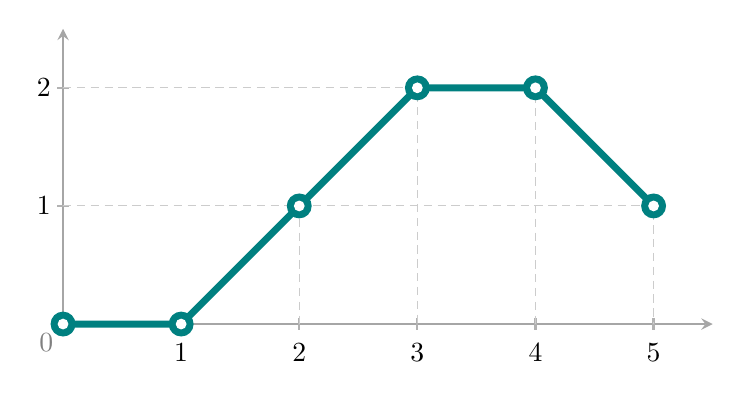
\begin{tikzpicture}[scale=1.5, >=stealth]
    \draw[thick, ->, gray!70] (0,0) -- (5.5,0);
    \draw[thick, ->, gray!70] (0,0) -- (0,2.5);
    
    \node[below left, gray] at (0,0) {0};
    \draw[thick, gray!60] (-0.05,1) -- (0.05,1) node[left=0.1cm, black] {1};
    \draw[thick, gray!60] (-0.05,2) -- (0.05,2) node[left=0.1cm, black] {2};
    
    \foreach \x in {1,2,3,4,5} {
        \draw[thick, gray!60] (\x,-0.05) -- (\x,0.05);
        \node[below=0.12cm] at (\x,0) {\x};
    }
    
    \draw[densely dashed, gray!40, thin] (0,1) -- (2,1) -- (2,0);
    \draw[densely dashed, gray!40, thin] (0,2) -- (3,2) -- (3,0);
    \draw[densely dashed, gray!40, thin] (3,2) -- (4,2) -- (4,0);
    \draw[densely dashed, gray!40, thin] (2,1) -- (5,1) -- (5,0);
    
    \draw[teal, line width=2.5pt, line join=round, line cap=round] (0,0) -- (1,0) -- (2,1) -- (3,2) -- (4,2) -- (5,1);
    
    \foreach \p in {(0,0), (1,0), (2,1), (3,2), (4,2), (5,1)} {
        \fill[teal] \p circle (3pt);
        \fill[white] \p circle (1.3pt);
    }
\end{tikzpicture}

\end{center}

\begin{itemize}
    \item \textbf{Truy vấn \texttt{[1,5]}:}  
    Các bước đi: $1 \to 2$, $2 \to 3$, $3 \to 4$, $4 \to 5$  
    Quãng đường = $\sqrt{2} + \sqrt{2} + 1 + \sqrt{2} = 3\sqrt{2} + 1 = 5.242641$

    \item \textbf{Truy vấn \texttt{[2,4]}:}  
    Các bước đi: $2 \to 3$, $3 \to 4$  
    Quãng đường = $\sqrt{2} + 1 = 2.414214$
\end{itemize}

\end{explain}